\section{Accessibilità}
\subsection{Navigazione}
Per evitare il disorientamento dell'utente in ogni pagina è stato aggiunto ad ogni pagina una barra (breadcrumb) dove è riportato il nome della pagina e la gerarchia di pagine per arrivare ad essa.\newline 
\begin{figure}[h]
	\label{bc} 
	\centering % centra
	
\includegraphics[width=1\textwidth]{immagini/bc.png}
	\caption{Un esempio di breadcrumb per i dettagli prodotto} % descrizione
\end{figure} \mbox{} \\
Inoltre nella barra di navigazione viene disabilitato  il link alla pagina corrente evitando così link circolari.
\begin{figure}[h]
	\label{navbar} 
	\centering % centra
	
\includegraphics[width=1\textwidth]{immagini/navbar.png}
	\caption{In questo caso ci so trova sulla home e il link per andare alla home è disabilitato} % descrizione
\end{figure} \mbox{} \\
Visto che alcune pagine del sito sono liste che possono diventare molto lunghe abbiamo inserito un tasto per tornare in cima alla pagina.
\begin{figure}[h]
	\label{su} 
	\centering % centra
	
\includegraphics[width=0.2\textwidth]{immagini/su.png}
	\caption{Icona torna su} % descrizione
\end{figure} \mbox{} \\


\subsection{Scelta dei colori}
Per quanto riguarda la scelta dei colori da utilizzare, abbiamo fatto uso della Ruota dei colori accessibili per verificare ci fosse un constrasto abbastanza elevato tra i vari colori, in modo che anche le persone con disturbi visivi quali \emph{Deuteranopia} (insensibilità al verde), \emph{Protanopia} (insensibilità al rosso) e \emph{Tritanopia} (insensibilità al blu), siano in grado di distinguere chiaramente i testi e i link presenti in tutte le pagine del nostro sito.\newline
Abbiamo fatto riferimento alle WCAG (Web Content Accessibility Guidelines 2.0) che richiede un livello minimo di contrasto di 4.5:1, rispettato dai nostri accostamenti di colori.\newline
I colori utilizzati, oltre al classico bianco e nero, sono un grigio (\#CCCCCC) per lo sfondo della barra del menù e per i vari bordi degli elementi una tonalità di blu (\#004D66) con testo in bianco per i pulsanti; i colori dei link ancora da visitare sono visualizzati con lo stesso colore dello sfondo dei pulsanti (\#004D66) mentre per i link ancora già visitati il violetto (\#800080) già disponibile di default.
Grazie allo strumento fornitoci dal sito \emph{http://www.color-blindness.com/coblis-color-blindness-simulator/}, siamo in grado di mostrare come la pagina verrebbe vista da persone affette dai precedenti disturbi visivi, risultando comunque chiara e leggibile.\newline


\mbox{} \\ \mbox{} \\ \Spazio

\begin{figure}[h]
	\label{originale}
	\centering %centra
	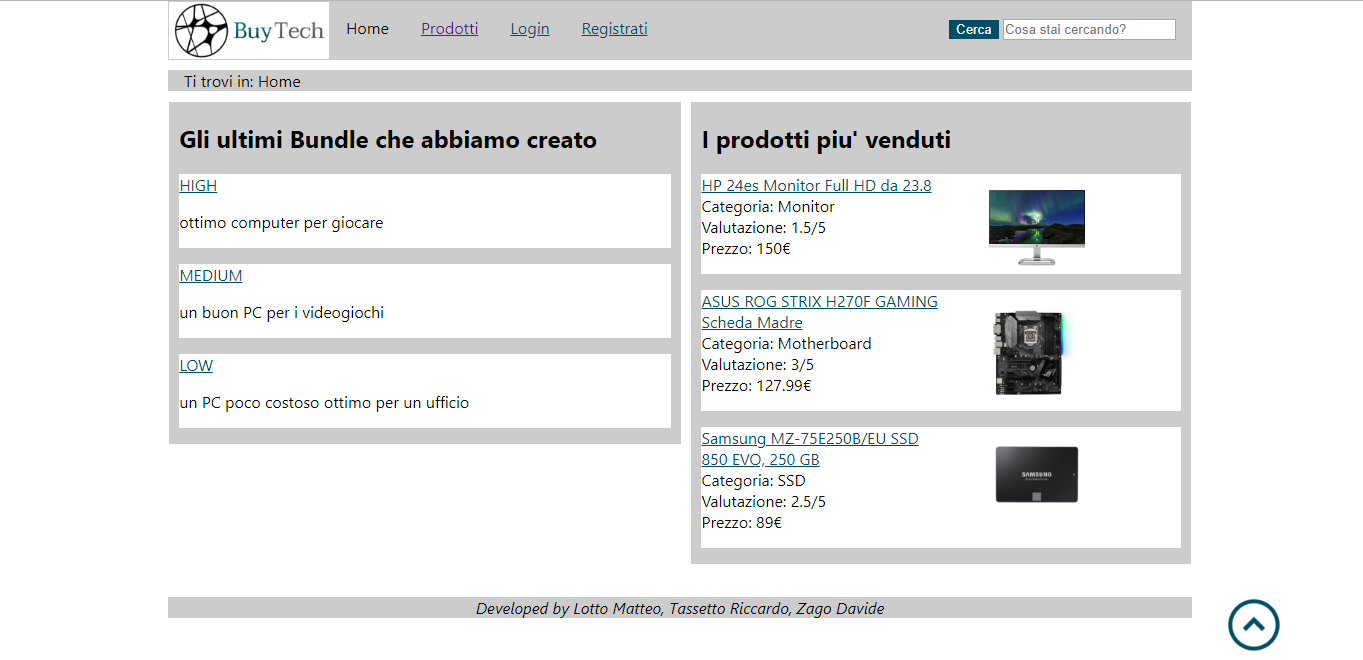
\includegraphics[width=1\textwidth]{immagini/screenhome.png}
	\caption{Originale} %descrizione
\end{figure}


\begin{figure}[h]
	\label{deuteranopia}
	\centering %centra
	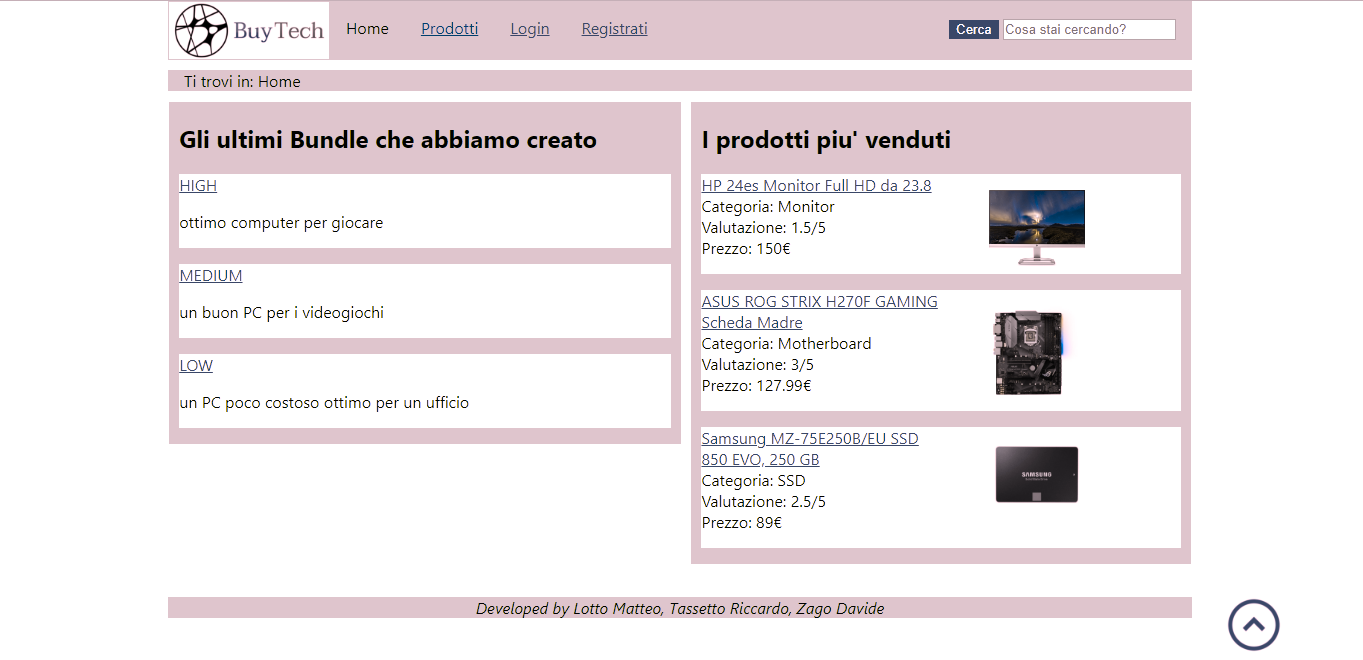
\includegraphics[width=1\textwidth]{immagini/homedeute.png}
	\caption{Deuteranopia} %descrizione
\end{figure}\mbox{} \\

\mbox{} \\ \mbox{} \\ \Spazio
\newline
\begin{figure}[h]
	\label{protanopia}
	\centering %centra
	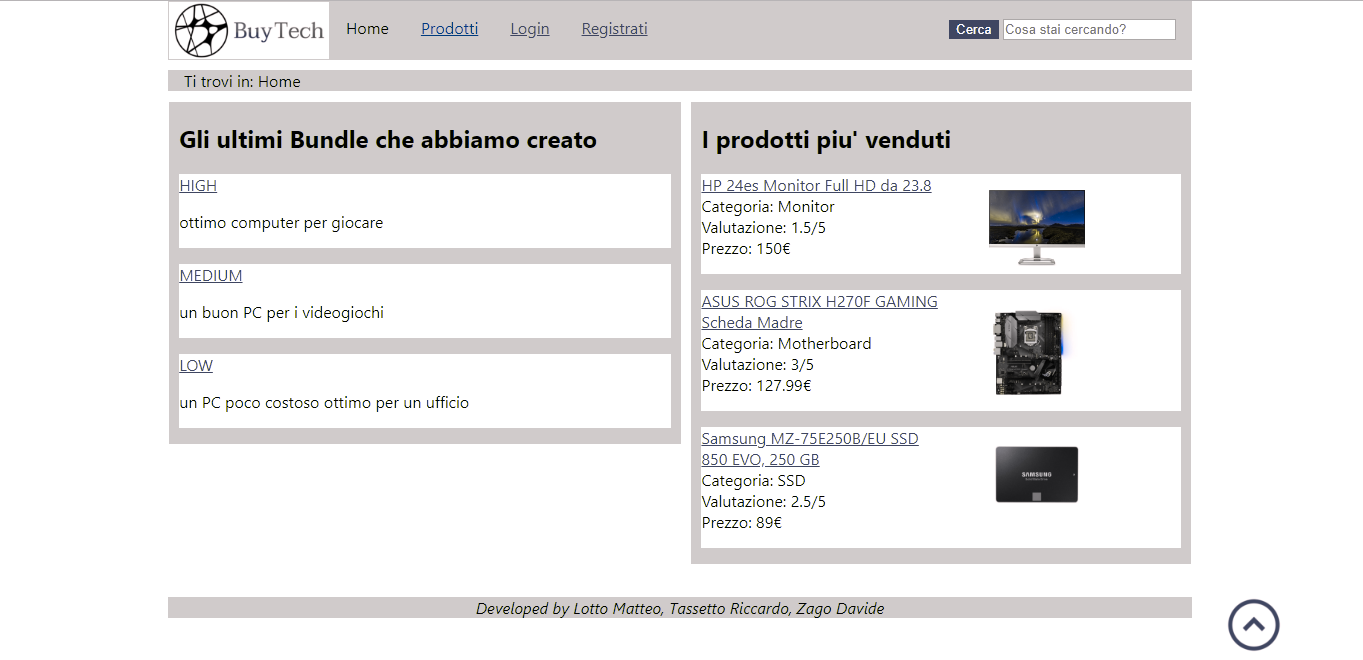
\includegraphics[width=1\textwidth]{immagini/homeprota.png}
	\caption{Protanopia} %descrizione
\end{figure}

\mbox{} \\ \mbox{} \\ \Spazio
\newline
\begin{figure}[h]
	\label{tritanopia}
	\centering %centra
	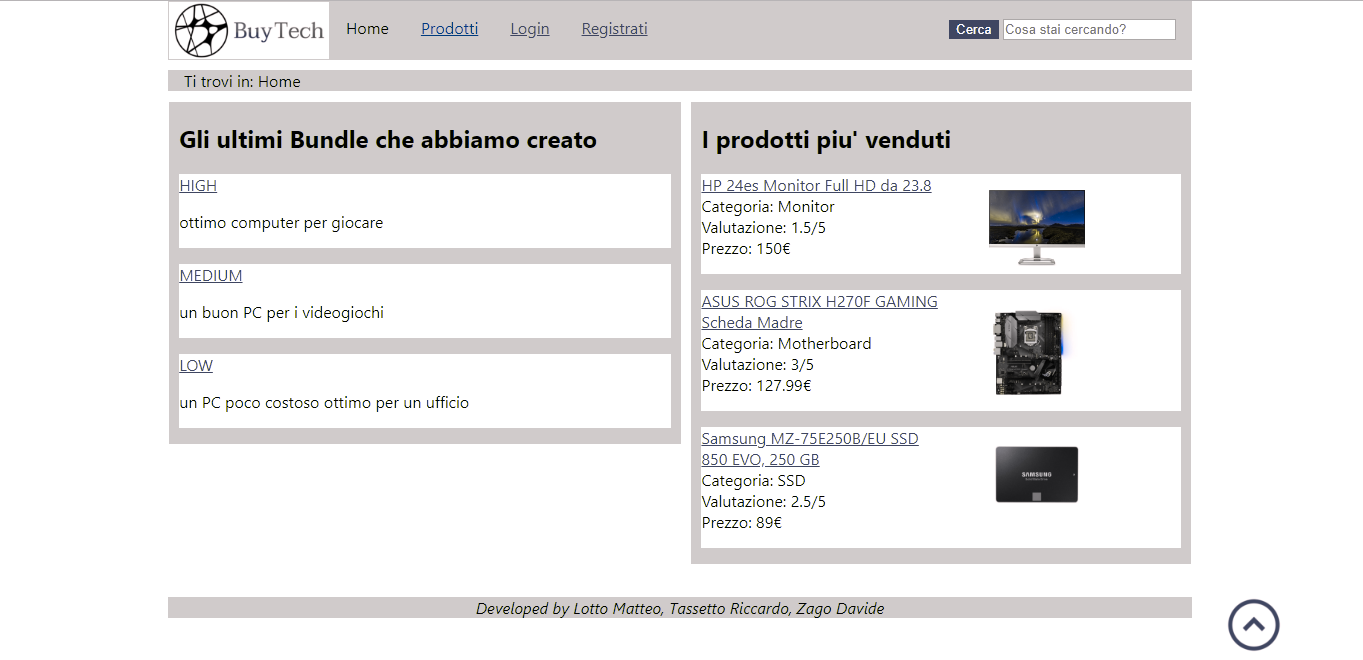
\includegraphics[width=1\textwidth]{immagini/hometrita.png}
	\caption{Tritanopia} %descrizione
\end{figure}
\newline
